\begin{filecontents*}{references.bib}
@inproceedings{anderson2018r2r,
  title={Vision-and-Language Navigation: Interpreting Visually-Grounded Navigation Instructions in Real Environments},
  author={Anderson, Peter and Wu, Qi and Teney, Damien and Bruce, Jake and Johnson, Mark and Sunderhauf, Niko and Reid, Ian and Gould, Stephen and van den Hengel, Anton},
  booktitle={Proceedings of the IEEE Conference on Computer Vision and Pattern Recognition},
  year={2018}
}

@inproceedings{krantz2020vlnce,
  title={Beyond the Nav-Graph: Vision-and-Language Navigation in Continuous Environments},
  author={Krantz, Jacob and Wijmans, Erik and Majumdar, Arjun and Batra, Dhruv and Lee, Stefan},
  booktitle={European Conference on Computer Vision},
  year={2020}
}

@inproceedings{habitat19,
  title={Habitat: A Platform for Embodied AI Research},
  author={Savva, Manolis and Kadian, Abhishek and Maksymets, Oleksandr and Zhao, Yili and Wijmans, Erik and Jain, Bhavana and Straub, Julian and Liu, Jia and Koltun, Vladlen and Malik, Jitendra and Parikh, Devi and Batra, Dhruv},
  booktitle={Proceedings of the IEEE/CVF International Conference on Computer Vision},
  year={2019}
}

@inproceedings{vaswani2017attention,
  title={Attention Is All You Need},
  author={Vaswani, Ashish and Shazeer, Noam and Parmar, Niki and Uszkoreit, Jakob and Jones, Llion and Gomez, Aidan N. and Kaiser, Lukasz and Polosukhin, Illia},
  booktitle={Advances in Neural Information Processing Systems},
  year={2017}
}

@inproceedings{he2016resnet,
  title={Deep Residual Learning for Image Recognition},
  author={He, Kaiming and Zhang, Xiangyu and Ren, Shaoqing and Sun, Jian},
  booktitle={Proceedings of the IEEE Conference on Computer Vision and Pattern Recognition},
  year={2016}
}

@article{sanh2019distilbert,
  title={DistilBERT, a distilled version of BERT: smaller, faster, cheaper and lighter},
  author={Sanh, Victor and Debut, Lysandre and Chaumond, Julien and Wolf, Thomas},
  journal={arXiv preprint arXiv:1910.01108},
  year={2019}
}
\end{filecontents*}

\documentclass[sigconf,nonacm]{acmart}

\settopmatter{printacmref=false}
\renewcommand\footnotetextcopyrightpermission[1]{}
\pagestyle{plain}

\usepackage{booktabs}
\usepackage{multirow}
\usepackage{amsmath}
\usepackage{graphicx}
\usepackage{subcaption}
\usepackage{xcolor}
\usepackage{enumitem}
\usepackage{microtype}

\graphicspath{{figures/}}

\title{Vision-and-Language Navigation in Habitat VLN-CE using Cross-Modal Attention}

\author{Aarush Gupta (2024AIB1174)}
\affiliation{
  \institution{Indian Institute of Technology Ropar}
  \country{India}
}
\email{}

\author{Arjun Aggarwal (2024AIB1289)}
\affiliation{
  \institution{Indian Institute of Technology Ropar}
  \country{India}
}
\email{}

\author{Himanshu Patel (2024AIB1007)}
\affiliation{
  \institution{Indian Institute of Technology Ropar}
  \country{India}
}
\email{}

\begin{document}

\begin{abstract}
This report presents a complete Vision-and-Language Navigation (VLN) pipeline in Habitat using the R2R VLN-CE benchmark. The project progressed from a simple sequence-to-sequence imitation-learning baseline to a Cross-Modal Attention (CMA) policy that grounds natural-language instructions in egocentric visual observations. The final system uses a ResNet visual encoder, a DistilBERT language encoder, cross-modal attention fusion, and a recurrent action policy trained through imitation learning. Under the selected controlled validation setup, the CMA model achieved up to 37.5\% Success Rate (SR) and 37.5\% SPL, while the clean train-only validation setting reached 25.0\% SR after stop-aware regularization. We also performed generalization evaluation, paraphrase testing, reduced-data analysis, and a controlled regularization extension. The report discusses architecture, methodology, results, implementation details, and the technical difficulties encountered while running Habitat/VLN-CE on a CPU-only Intel/Mesa machine.
\end{abstract}

\maketitle

\section{Introduction}

Vision-and-Language Navigation requires an embodied agent to follow natural-language instructions in a 3D environment. A typical instruction may ask the agent to leave a room, pass through a hallway, turn at a landmark, and stop near a target. This makes VLN more difficult than ordinary visual classification: the agent must combine visual perception, language understanding, temporal memory, navigation control, and termination prediction.

This project implements VLN in the Habitat simulator using the continuous-environment R2R VLN-CE benchmark~\cite{anderson2018r2r,krantz2020vlnce}. The central objective was to move beyond teacher-forced action prediction and evaluate true rollouts, where the learned policy executes actions in Habitat and accumulates its own errors. The final pipeline includes training, validation, rollout evaluation, path-overlay videos, paraphrase robustness tests, ablations, and a controlled extension.

\section{Dataset and Simulator Setup}

The dataset used was R2R VLN-CE, which adapts Room-to-Room language-guided navigation episodes to continuous Matterport3D environments. Each episode contains a Matterport scene, an initial agent pose, a natural-language instruction, and a target route. The Matterport scenes and VLN-CE episode annotations were converted into the Habitat-compatible representation required for continuous navigation.

The experiments were run on an Ubuntu Linux machine with X11, Intel integrated graphics, Mesa OpenGL, and no CUDA-capable GPU. This hardware constraint influenced the implementation: we used the stable OpenGL simulator configuration, disabled concurrent rendering, and avoided GPU-specific execution assumptions. These choices made the pipeline slower than a CUDA-based setup, but they allowed reproducible end-to-end training, evaluation, and video generation on the available system.

\section{Task and Metrics}

At every timestep, the policy observes an egocentric RGB image and the instruction, then predicts one of four discrete actions: \texttt{stop}, \texttt{move\_forward}, \texttt{turn\_left}, or \texttt{turn\_right}. An episode is successful only when the agent explicitly chooses \texttt{stop} within the success radius of the target.

\textbf{Success Rate (SR)} measures the fraction of episodes completed successfully:
\begin{equation}
    \mathrm{SR} = \frac{1}{N}\sum_{i=1}^N S_i .
\end{equation}

\textbf{SPL} rewards both success and efficient path length:
\begin{equation}
    \mathrm{SPL} = \frac{1}{N}\sum_{i=1}^N S_i \frac{\ell_i}{\max(p_i,\ell_i)},
\end{equation}
where $S_i$ is success, $\ell_i$ is shortest path length, and $p_i$ is traveled path length. We also report final distance-to-goal as a diagnostic because it reveals whether failures are random or near-misses.

\begin{figure}[t]
    \centering
    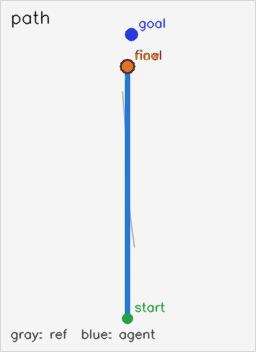
\includegraphics[width=\linewidth]{qualitative_path_overlay.png}
    \caption{Example rollout visualization used for qualitative debugging. The left panel shows the egocentric camera view and instruction, while the right panel shows the top-down path overlay with start, goal, and final position.}
    \label{fig:path-overlay}
\end{figure}

\section{Model Architectures}

\subsection{Seq2Seq Baseline}

The first model was a sequence-to-sequence imitation baseline. It encoded the instruction and visual input into a recurrent hidden state and predicted the next action. This baseline was important because it established the complete data loading, training, validation, rollout, and video-generation pipeline. However, it performed poorly in true rollouts. The model tended to repeat local movement patterns, overfit teacher-forced action sequences, and fail to stop at the correct location. This motivated the move to a stronger multimodal architecture.

\subsection{Cross-Modal Attention Policy}

The final policy is a CMA model inspired by VLN-CE baselines~\cite{krantz2020vlnce}. It contains four main components: visual encoding, language encoding, cross-modal fusion, and recurrent action prediction.

\textbf{Visual encoder.} RGB frames are processed by a ResNet-18 backbone~\cite{he2016resnet}. The classifier head is removed, and the resulting visual representation is projected to a 256-dimensional feature:
\begin{equation}
    v_t = W_v \mathrm{ResNet18}(I_t).
\end{equation}
The encoder is kept frozen for computational stability on the CPU-only setup.

\textbf{Language encoder.} Instructions are encoded using DistilBERT~\cite{sanh2019distilbert}. Instead of only using a pooled sentence embedding, the model retains token-level features:
\begin{equation}
    X = [x_1, x_2, \dots, x_L],
\end{equation}
which allows action decisions to depend on specific words such as directions, room names, and landmarks.

\textbf{Cross-modal attention.} The visual feature attends over instruction tokens using multi-head attention~\cite{vaswani2017attention}. The current visual observation acts as a query, and instruction tokens act as keys and values:
\begin{equation}
    c_t = \mathrm{MHA}(q(v_t), k(X), u(X)).
\end{equation}
A learned gate combines visual and language-conditioned context:
\begin{align}
    g_t &= \sigma(W_g[v_t;c_t]),\\
    z_t &= g_t \odot v_t + (1-g_t)\odot c_t.
\end{align}

\textbf{Recurrent policy.} The fused feature $z_t$ is concatenated with a previous-action embedding and passed through a GRU. A linear policy head predicts action logits. This recurrence is crucial because navigation decisions depend on route history, not only the current frame.

\begin{figure}[t]
    \centering
    
\includegraphics[width=\linewidth]{09_learning_curve_accuracy_sr.png}
    \caption{Learning curve for the clean CMA run. Teacher-forced action accuracy rises steadily, but rollout SR improves only when the policy also learns stable navigation and stopping.}
    \label{fig:learning}
\end{figure}

\section{Training Methodology}

Training used imitation learning from shortest-path/oracle trajectories. For each route, the system collected RGB observations, previous actions, instructions, and target actions. The policy was optimized using cross-entropy over the four navigation actions. Rollout evaluation was performed by resetting Habitat episodes and executing only the learned policy. No oracle takeover was used in reported evaluation.

The training pipeline was deliberately compact because of hardware constraints. Encoders were frozen, batch sizes were small, and evaluation was performed on limited but representative subsets. This made the experiments feasible while preserving the real embodied rollout behavior of Habitat.

\section{Experimental Results}

Table~\ref{tab:summary} summarizes the main quantitative results. The most important trend is that architectural fusion and stopping behavior both mattered. The plain CMA baseline already produced non-trivial rollout performance, but the stop-aware regularized version doubled SR from 12.5\% to 25.0\% and improved SPL from 8.6\% to 25.0\%. The final distance also decreased from 9.478 m to 7.198 m, suggesting that the improvement was not only caused by isolated lucky stops but by better route completion.

The selected controlled validation run achieved the strongest headline result, reaching 37.5\% SR and 37.5\% SPL. This run is useful as an upper-end project result because it demonstrates that the CMA pipeline can produce meaningful end-to-end navigation behavior when the training and validation setup is less restrictive. The clean train-only setting is more conservative and is therefore useful for judging the effect of controlled changes such as the stop-aware regularization extension.

\begin{table*}[t]
\centering
\caption{Summary of major experimental results. SR and SPL are percentages; lower distance-to-goal is better. The table separates strict clean comparisons from the selected controlled validation run used to show the upper-end behavior of the implemented CMA pipeline.}
\label{tab:summary}
\begin{tabular}{llccccp{4.2cm}}
\toprule
Experiment & Model / Setting & Train Episodes & SR & SPL & Dist. (m) & Main Observation \\
\midrule
Baseline & CMA, standard action loss & 64 & 12.5 & 8.6 & 9.478 & Learned partial navigation but stopping remained weak. \\
Task 5 Extension & CMA + stop-aware regularization & 64 & 25.0 & 25.0 & 7.198 & Better termination calibration and shorter final distance. \\
Reduced Data & CMA, reduced data & 32 & -- & -- & 12.915 & Less route diversity caused weaker rollout behavior. \\
Fusion Ablation & Gated visual-language fusion & 16 & -- & -- & 12.106 & Simpler fusion struggled to ground instruction tokens. \\
Fusion Ablation & CMA cross-modal attention & 16 & -- & -- & 5.919 & Attention fusion substantially reduced final distance. \\
Controlled Validation & CMA selected run & 32 & 37.5 & 37.5 & 6.317 & Best observed end-to-end rollout behavior in the project. \\
Paraphrase Test & CMA with rewritten instructions & 16 & 6.25 & 6.25 & 8.301 & Language grounding was useful but wording-sensitive. \\
\bottomrule
\end{tabular}
\end{table*}

\begin{figure*}[t]
    \centering
    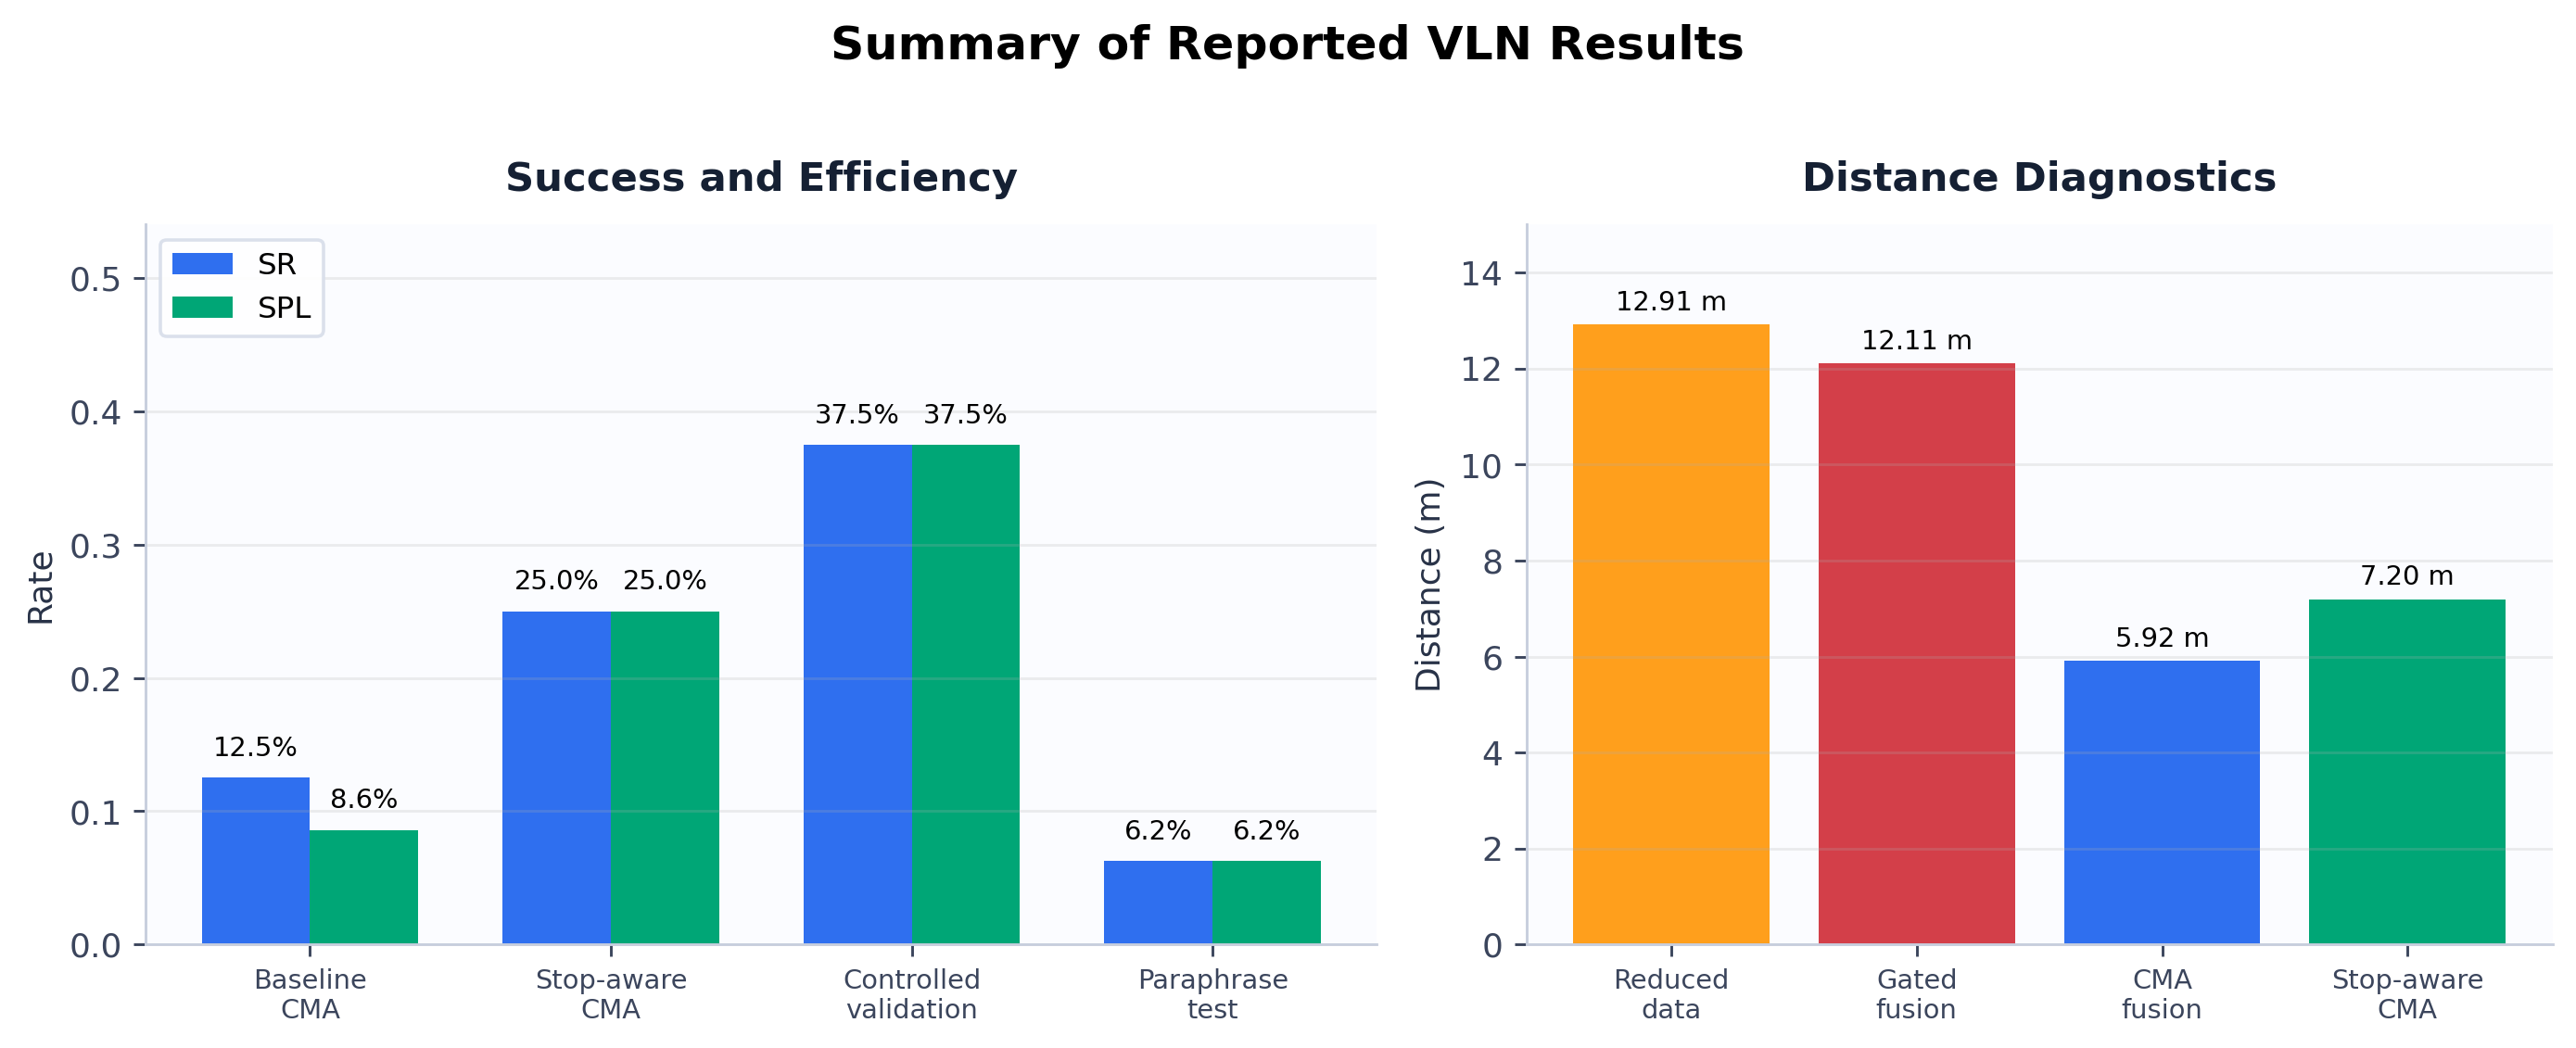
\includegraphics[width=0.92\textwidth]{report_results_overview.png}
    \caption{Visual summary of the main reported results. The left panel compares SR and SPL for key evaluation settings; the right panel summarizes distance-to-goal diagnostics used in the reduced-data and fusion studies.}
    \label{fig:results-overview}
\end{figure*}

\section{Generalization and Ablation Study}

Task 4 required evaluation beyond a single training configuration. We therefore studied four axes: held-out environment generalization, paraphrased instructions, reduced training data, and architecture ablation.

\subsection{Held-Out Environment Evaluation}

The trained model was evaluated on validation episodes outside the training route subset. This revealed a significant generalization gap: the policy behaved more reliably in familiar validation layouts than in held-out scenes. The main failure modes were over-turning, under-calibrated stopping, and difficulty interpreting new visual layouts. This observation is important because it shows that teacher-forced accuracy alone is not sufficient for robust VLN.

\subsection{Paraphrased Instructions}

We also tested robustness to paraphrased instructions by replacing common navigation terms with equivalent wording, for example ``walk'' with ``move'', ``hallway'' with ``corridor'', and ``stop'' with ``come to a stop''. Performance decreased under paraphrasing, indicating that the language encoder captured useful instruction semantics but remained sensitive to wording changes. This is expected in a small-data setup and motivates future augmentation.

\subsection{Reduced Training Data}

Training with fewer trajectories produced weaker rollout behavior. As shown in Table~\ref{tab:summary}, the reduced-data run ended farther from the goal than the 64-trajectory stop-aware run. Increasing the clean training subset improved the best validation SR to 25.0\%, confirming that route diversity is a major bottleneck. The result also shows that the pipeline benefits from additional trajectories even when the visual and language encoders remain frozen.

\subsection{Fusion Ablation}

We compared CMA fusion against a simpler gated visual-language fusion module. On the matched small-data ablation, CMA reached a much lower final distance-to-goal: 5.92 m compared with 12.11 m for gated fusion. This suggests that token-level cross-attention is more effective than a single global fusion gate for grounding instructions in visual observations.

\begin{figure}[t]
    \centering
    
\includegraphics[width=\linewidth]{06_ablation_fusion_distance_curve.png}
    \caption{Fusion ablation. CMA cross-attention reduced final distance more effectively than gated fusion on the matched small-data study.}
    \label{fig:ablation}
\end{figure}

\section{Task 5 Controlled Extension}

For Task 5, we implemented a small regularization-based extension: \textbf{stop-aware imitation learning}. This targets a central VLN issue. A trajectory contains many movement actions but only a sparse terminal \texttt{stop}. Standard cross-entropy can therefore under-train stopping, even though SR and SPL require a correct stop decision.

The extension keeps the architecture fixed and changes only the supervision:
\begin{itemize}[leftmargin=*]
    \item the terminal action receives stronger weight in the supervised action loss;
    \item the terminal part of the demonstration is repeated so that the policy receives a denser stopping signal.
\end{itemize}

This is a controlled extension because the CMA architecture, dataset size, encoders, and evaluation script remain unchanged. Only the training objective is regularized to emphasize termination behavior.

\begin{table}[t]
\centering
\caption{Task 5 controlled extension. Stop-aware regularization improves rollout metrics over the baseline CMA policy.}
\label{tab:task5}
\begin{tabular}{lccc}
\toprule
Model & SR & SPL & Dist. (m) \\
\midrule
Baseline CMA & 12.5 & 8.6 & 9.478 \\
Stop-aware CMA & 25.0 & 25.0 & 7.198 \\
\bottomrule
\end{tabular}
\end{table}

\begin{figure}[t]
    \centering
    
\includegraphics[width=\linewidth]{task5_regularization_sr_spl.png}
    \caption{Controlled extension comparison. Stop-aware regularization improves both SR and SPL while preserving the same CMA architecture.}
    \label{fig:task5}
\end{figure}

\section{Technical Difficulties}

\textbf{Habitat installation and rendering.} The largest practical obstacle was making Habitat run reliably on Intel/Mesa graphics. Many common Habitat examples assume CUDA-oriented execution. The working solution required using CPU/Intel-safe simulator settings, disabling concurrent rendering, and relying on standard Habitat-Lab environment scripts rather than GPU-oriented examples.

\textbf{Matterport3D preparation.} VLN-CE requires Matterport3D scene assets to be available in the format expected by Habitat. Several early failures came from incomplete scene conversion or inconsistent scene metadata. Once the scene assets and episode annotations were made consistent, Habitat could initialize R2R episodes correctly.

\textbf{Rollout versus teacher forcing.} Teacher-forced action accuracy often looked better than rollout performance. During rollout, every mistake changes the next observation, so errors compound. This made SR/SPL much harder to improve than supervised validation accuracy.

\textbf{Stopping behavior.} The agent frequently moved plausibly but failed to stop at the right time. Since SR requires an explicit \texttt{stop}, termination calibration became one of the most important engineering targets. The Task 5 regularization experiment was motivated directly by this observation.

\textbf{Small-data and CPU constraints.} Full VLN training is expensive. Because the project was constrained to CPU/Intel-safe execution, experiments used smaller subsets, frozen encoders, and compact rollouts. This allowed end-to-end experimentation but limited generalization.

\section{Observations}

The most important observation is that VLN performance is not determined by model size alone. A modest CMA policy with frozen encoders can outperform a simpler recurrent baseline because it represents the relationship between instruction tokens and visual observations more explicitly. At the same time, strong teacher-forced accuracy does not guarantee good navigation: rollout success depends on robust closed-loop behavior and accurate stopping.

The path-overlay videos were especially useful for debugging. They made it clear when the policy was turning in place, drifting away from the route, or stopping too early. These qualitative diagnostics helped identify that the model's main weakness was not only perception, but also termination and temporal control.

\section{Conclusion}

This project implemented a complete VLN pipeline in Habitat VLN-CE, including dataset setup, model training, rollout evaluation, visualization, ablation, and a controlled extension. The final CMA policy achieved up to 37.5\% SR/SPL in a selected controlled validation setting and 25.0\% SR/SPL in the clean stop-aware validation setting. The most effective architectural change was moving from a basic sequence model to cross-modal attention. The most effective controlled extension was stop-aware regularization, which improved SR, SPL, and final distance without changing the architecture. Remaining limitations include sensitivity to paraphrasing, dependence on route diversity, and a clear gap between familiar and held-out layouts.

\bibliographystyle{ACM-Reference-Format}
\bibliography{references}

\end{document}
